\documentclass{beamer}
\usetheme{Antibes}
\setbeamertemplate{navigation symbols}{} 
\usepackage{amsmath}
\usepackage[T1]{fontenc}
\usepackage{lmodern}

\usepackage{graphicx}
\graphicspath{{.}{images/}}

\begin{document}

\title[Optical Nonlinear Spectroscopy of Gold and Silicon Nanoparticles\hspace{5.5cm}\insertframenumber/\inserttotalframenumber]{Optical Nonlinear Spectroscopy of Gold and Silicon Nanoparticles\vspace{-5pt}}
\author{Sean M. Anderson\vspace{-7pt}}
\institute{Centro de Investigaciones en \'Optica, A.C\vspace{-10pt}}
\date{January 30, 2012\vspace{-17pt}}
\titlegraphic{
\begin{figure}
%\includegraphics[height=0.47\textheight]{restricted/fluor}
\end{figure}}

\begin{frame}
\titlepage
\end{frame}

\begin{frame}
When you combine\ldots
\begin{center}
\begin{figure}
%\includegraphics[height=0.4\textheight]{restricted/vulcan}
\end{figure}
\end{center}
with these\ldots
\begin{center}
\begin{figure}
%\includegraphics[height=0.4\textheight]{restricted/goldnps}
\end{figure}
\end{center}
\end{frame}


%--------------------------- Introduction -----------------------------%
\section*{Introduction}
\subsection*{Nanoparticles}
\begin{frame}
\begin{figure}
\centering
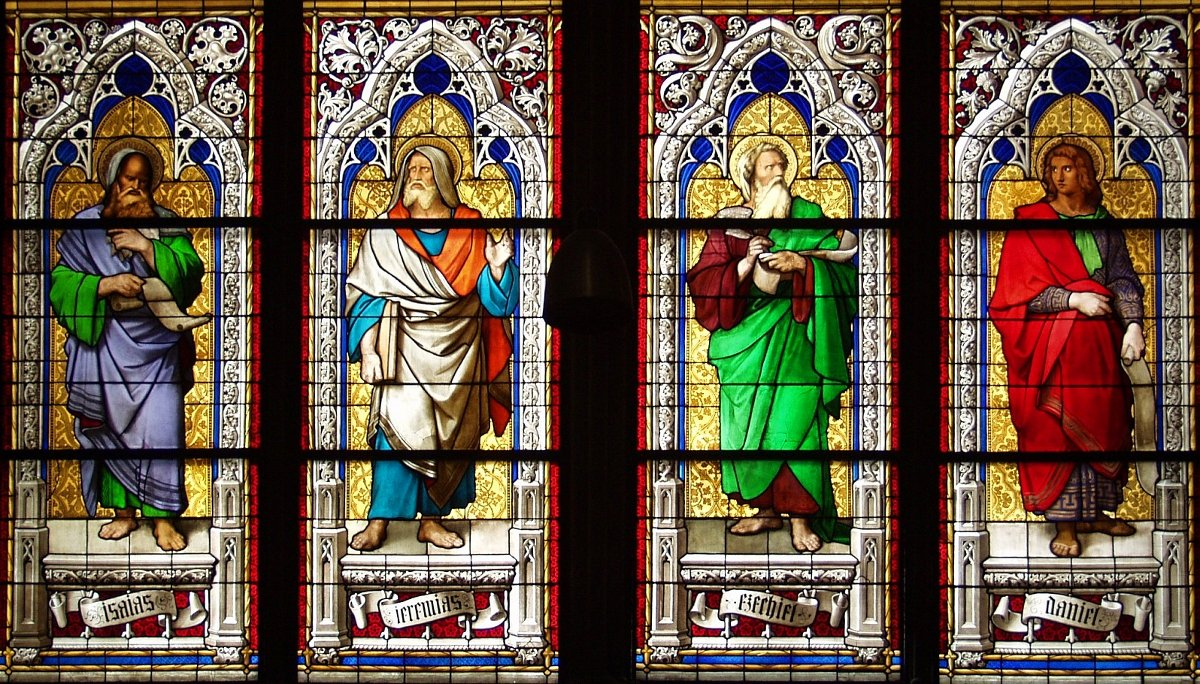
\includegraphics[width=\textwidth]{stained}
\end{figure}
\begin{center}
Historic use of metallic nanoparticles.\footnote{Image: Raimond Spekking.}
\end{center}
\end{frame}

\begin{frame}
\begin{figure}
\centering
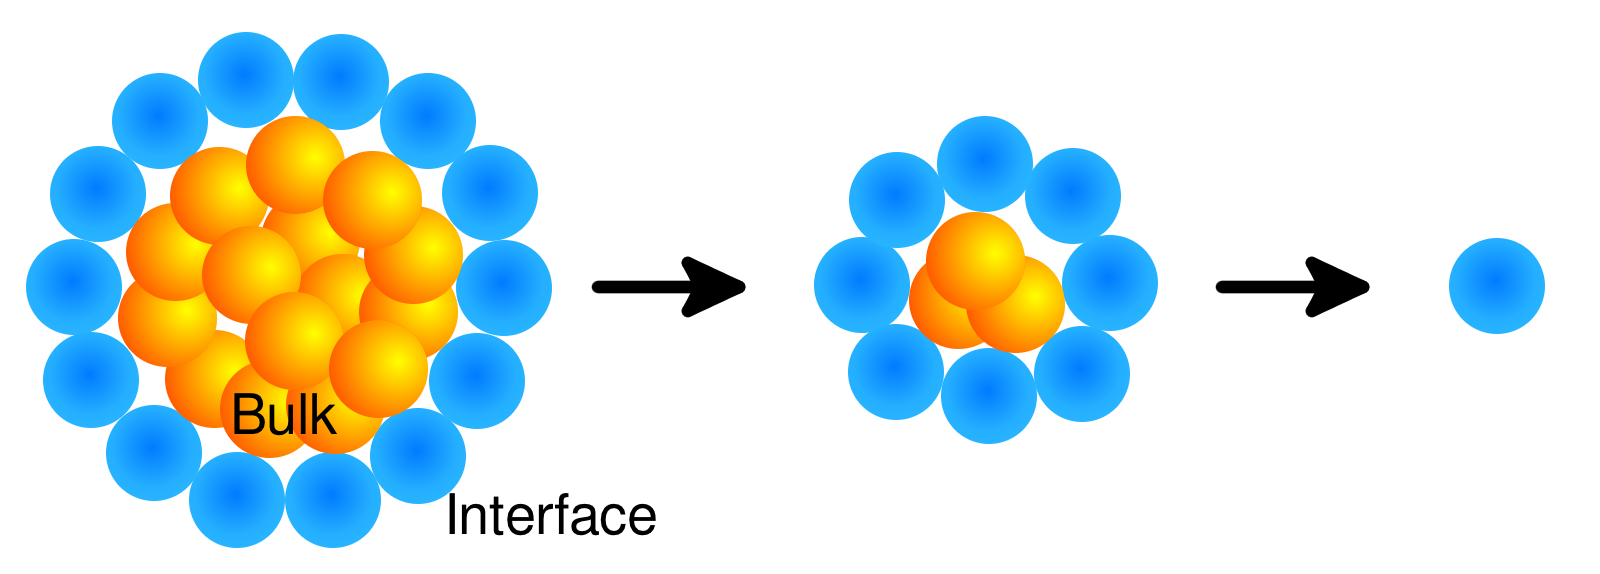
\includegraphics[width=\textwidth]{atoms}
\end{figure}
\begin{center}
Nanoparticles have large surface to volume ratios.
\end{center}
\end{frame}

\subsection{Our Samples}
\begin{frame}
\frametitle{Our Samples\footnote{Provided by Dr. Alejandro Reyes and Dr. Alicia Oliver of the IF-UNAM.}}
\begin{columns}
\column{0.5\textwidth}
\begin{itemize}
\item Created via ion implantation
\item Implanted on Suprasil 300 substrate
\item $8\times8$ and $8\times4$ mm transparent samples
\end{itemize}
\column{0.5\textwidth}
\begin{figure}
\centering
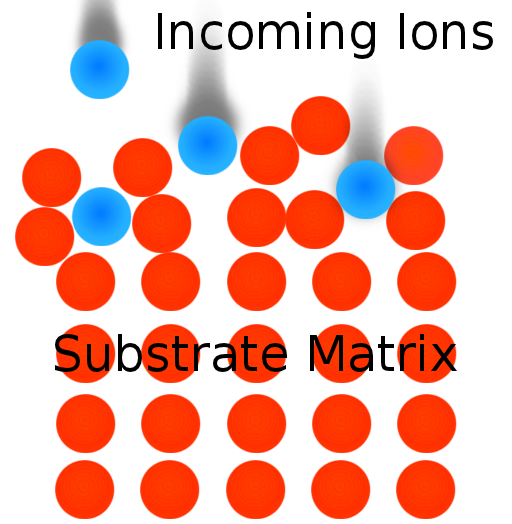
\includegraphics[width=\textwidth]{ions}
\end{figure}
\end{columns}
\end{frame}

\begin{frame}
\frametitle{Au Sample}
\begin{columns}
\column{0.5\textwidth}
\begin{figure}
\centering
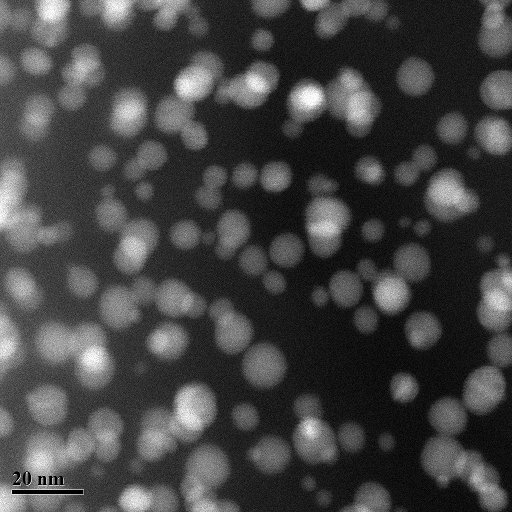
\includegraphics[width=\textwidth]{tem_au}
\end{figure}
\begin{center}
TEM scan.
\end{center}
\column{0.55\textwidth}
\begin{block}{Specifications}
\begin{itemize}
\item Size: $\sim$ 3 nm
\item Density: $5.8\times 10^{16}\,\,\text{nps}/\text{cm}^{3}$
\item Dose: $3.1\times 10^{16}\,\,\text{atoms}/\text{cm}^{2}$
\item Implantation Energy: 2\,MeV
\end{itemize}
\end{block}
\end{columns}
\end{frame}

\begin{frame}
\frametitle{Au$^{2+}$ Sample}
\begin{columns}
\column{0.55\textwidth}
\begin{block}{Specifications}
\begin{itemize}
\item Size: $\sim$ 3 nm
\item Density: $9.8\times 10^{16}\,\,\text{nps}/\text{cm}^{3}$
\item Dose: $5.0\times 10^{16}\,\,\text{atoms}/\text{cm}^{2}$
\item Implantation Energy: 2\,MeV
\end{itemize}
\end{block}
\column{0.5\textwidth}
\begin{figure}
\centering
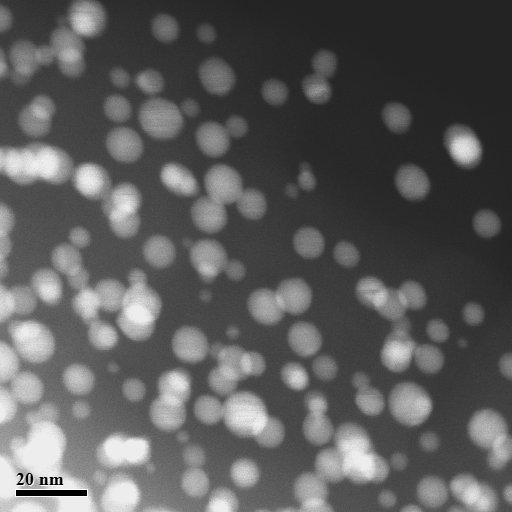
\includegraphics[width=\textwidth]{tem_aui}
\end{figure}
\begin{center}
TEM scan.
\end{center}
\end{columns}
\end{frame}

\begin{frame}
\frametitle{Si Sample}
\begin{columns}
\column{0.5\textwidth}
\begin{figure}
\centering
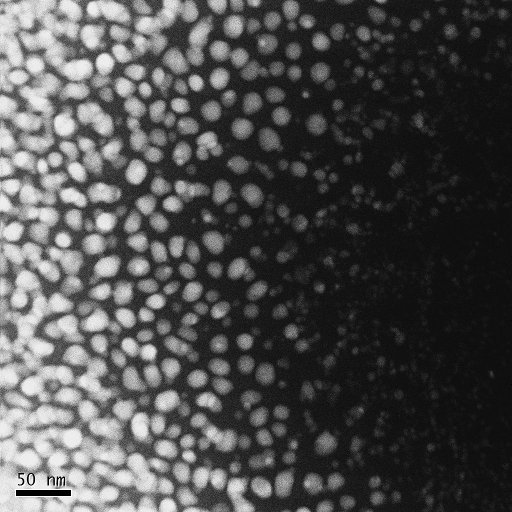
\includegraphics[width=\textwidth]{tem_si}
\end{figure}
\begin{center}
TEM scan.
\end{center}
\column{0.55\textwidth}
\begin{block}{Specifications}
\begin{itemize}
\item Size: $\sim$ 20 nm
\item Dose: $2.5\times 10^{17}\,\,\text{atoms}/\text{cm}^{2}$
\item Implantation Energy: 1.5\,MeV
\end{itemize}
\end{block}
\end{columns}
\end{frame}

\begin{frame}
\frametitle{Centrosymmetric Materials}
A centrosymmetric material is a material that displays inversion symmetry, such that $p(x,y,z)\rightarrow p(-x,-y,-z)$.
\begin{columns}
\column{0.5\textwidth}
\begin{figure}
\centering
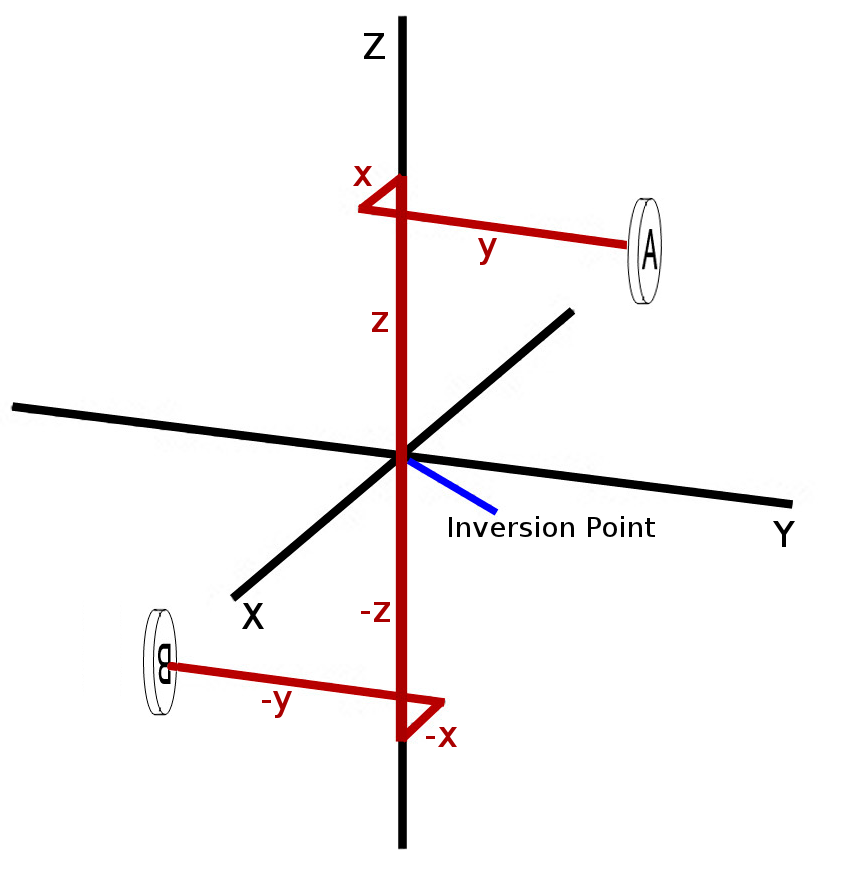
\includegraphics[width=\textwidth]{centro}
\end{figure}
\column{0.5\textwidth}
\begin{itemize}
\item Many nonlinear materials are centrosymmetric
\item Nanospheres are definitely centrosymmetric
\item The material in these nanoparticles is centrosymmetric
\end{itemize}
\end{columns}
\end{frame}

\subsection{Second-order Nonlinear Effects}
\begin{frame}
\frametitle{Second Harmonic Generation (SHG)}
\begin{block}{Characteristics\footnote{Image: Jon Chui}}
\begin{itemize}
\item Two photons of the same frequency combine
\item Create one photon of double the frequency
\end{itemize}
\end{block}
\begin{figure}
\centering
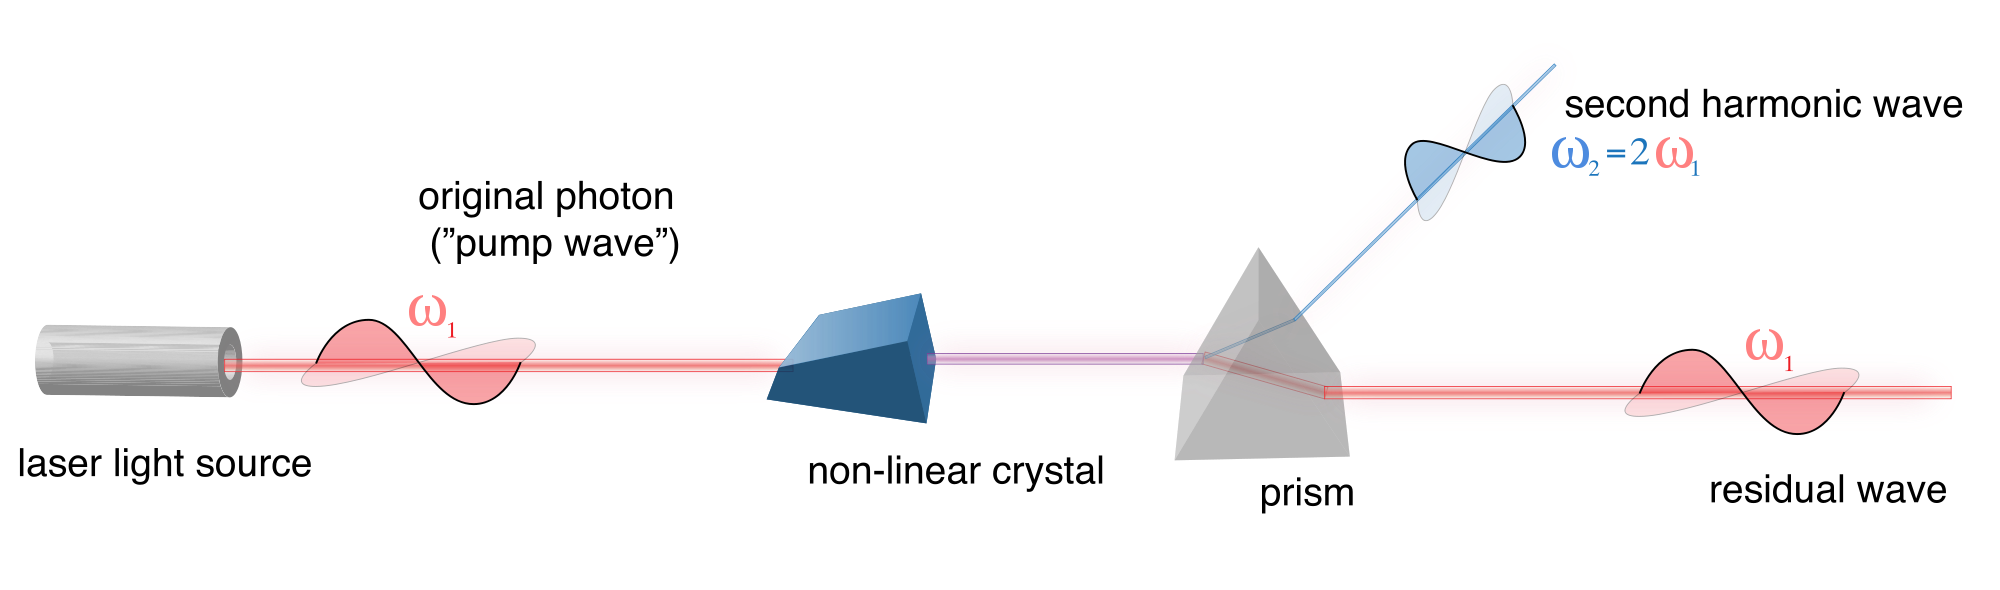
\includegraphics[width=0.9\textwidth]{shg}
\end{figure}
\end{frame}

\begin{frame}
\frametitle{Sum-frequency Generation (SFG)}
\begin{block}{Characteristics}
\begin{itemize}
\item Two photons of different frequency combine
\item Create one photon that is the sum of both frequencies
\end{itemize}
\end{block}
\begin{figure}
\centering
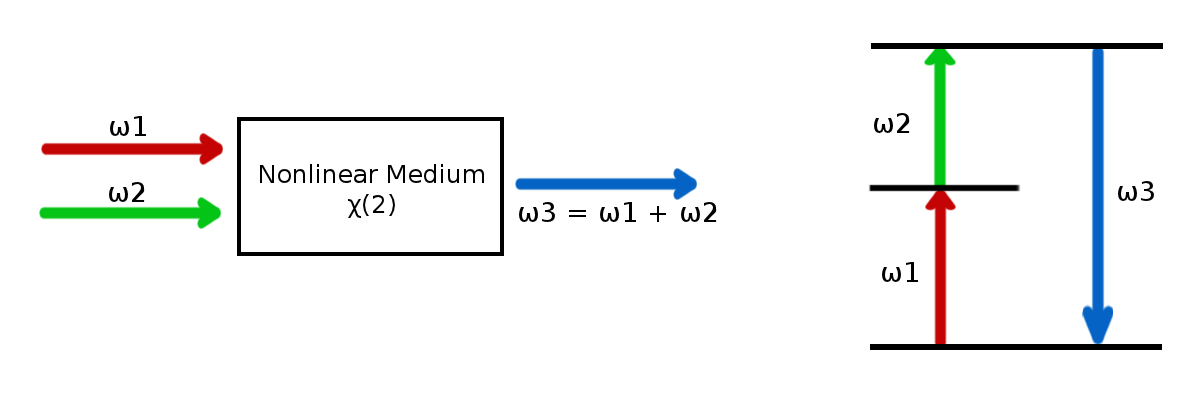
\includegraphics[width=\textwidth]{sfg}
\end{figure}
\end{frame}

\begin{frame}
\frametitle{Second-order Nonlinear Effects}
Early work\footnote{J.A. Armstrong et al. \emph{Physical Review}, 127(6):1918--1939, Sep 1962.} \footnote{N. Bloembergen et al. \emph{Physical Review}, 128(2):606--622, Oct 1962.} demonstrated that second-order processes
\begin{itemize}
\item Are dipole forbidden in the bulk of centrosymmetric materials
\item Are related to $\chi^{(2)}$, the nonlinear susceptibility
\item Have bigger dipolar (surface) than quadrupolar contributions
\end{itemize}\vfill
\begin{center}
Second-order processes are well studied for flat surfaces, but what about round materials like nanospheres?
\end{center}
\end{frame}

%------------------------------- Theory -------------------------------%
\section{Theory}
\subsection{Nonlinear Response of Nanoparticles}
\begin{frame}
\frametitle{Nonlinear Response of Nanoparticles}
\begin{itemize}
\item Early work\footnote{J.I. Dadap et al. \emph{Physical Review Letters}, 83(20):4045--4048, 1999.} \footnote{V.L. Brudny et al. \emph{Physical Review B}, 62(16):11152, 2000.} show that nanospheres have both dipolar and quadrupolar contributions
\item A few years later, Moch\'an et al.\footnote{W.L. Moch\'an et al. \emph{Physical Review B}, 68(8):085318, 2003.} determine the nonlinear polarization for an array of nanospheres.
\end{itemize}
\end{frame}

\begin{frame}
\frametitle{Theory}
The dipole moment for a single nanosphere is
\begin{equation}
\mathbf{p}^{(2)} = \gamma^{e}\mathbf{E}^{\text{ex}}(0)\cdot\nabla\mathbf{E}^{\text{ex}}(0) + \gamma^{m}\mathbf{E}^{\text{ex}}(0)\times\left[\nabla\times\mathbf{E}^{\text{ex}}(0)\right].\label{dipole}
\end{equation}
The quadrupole moment for a single nanoshpere is
\begin{equation}
\mathbf{Q}^{(2)} = \gamma^{q}\left(\mathbf{E}^{\text{ex}}(0)\mathbf{E}^{\text{ex}}(0) - \frac{1}{3}[\mathbf{E}^{\text{ex}}(0)]^{2}\,\mathbf{1}\right),\label{quad}
\end{equation}
where the $\gamma$'s are unknown nonlinear response functions. $\mathbf{p}^{(2)}$ is nonlocal because of the field derivative, while $\mathbf{Q}^{(2)}$ is local.
\end{frame}

\begin{frame}
The total nonlinear polarization for all the nanospheres is
\begin{equation}
\mathbf{P}^{nl} = n_{s}\mathbf{p}^{(2)} - \frac{1}{6}\nabla\cdot n_{s}\mathbf{Q}^{(2)},
\end{equation}
where $n_{s}$ is the nanocrystal volume density. We substitute equations \eqref{dipole} and \eqref{quad} to obtain
\begin{equation}
\mathbf{P}^{(2)} = \Delta^{\prime}\left(\mathbf{E}\cdot\nabla\mathbf{E}\right),\label{eq_mochan_p}
\end{equation}
where $\Delta^{'}\equiv n_{s}\left(\gamma^{e} - \gamma^{m} - \gamma^{q}/6\right)$ and represents a kind of bulk response function.
\end{frame}

\begin{frame}
\frametitle{Summary}
\begin{block}{Nonlinear response depends on}
\begin{itemize}
\item Nonlocal excitation of the electric dipole moment 
\item Local excitation of the electric quadrupole moment
\item The strength of the incident beam and
\item The form (plane wave, Gaussian beam, polarization, etc.)
\item The quadrupolar $\left(\mathbf{E}\cdot\nabla\right)\mathbf{E}$ term
\end{itemize}
\end{block}
What's the best way to enhance this signal?
\end{frame}

\subsection{The XP2SHG/SFG Technique}
\begin{frame}
\frametitle{The XP2SHG/SFG Technique}
\begin{itemize}
\item Early work\footnote{S. Cattaneo et al. \emph{Optics Letters}, 28(16):144--1447, 2003.} shows that using two cross-polarized beams reduces the number of unknown $\chi^{(2)}$ components
\item Wang et al. manage to discern surface and bulk contributions using two beams\footnote{F.X. Wang et al. \emph{Physical Review B}, 80(23):233402, 2009.}
\item Using two beams greatly increases the SHG/SFG signal usually enough to not need photon counters\footnote{P Figliozzi et al. \emph{Physical Review Letters}, 94(4):47401, 2005.}
\end{itemize}
\end{frame}

\begin{frame}
\frametitle{Theory}
The nonlinear polarization can be separated into two contributions\footnote{A. Wirth et al. \emph{Physica Status Solidi C}, 5(8):2662--2666, 2008.},
\begin{align}
\mathbf{P}^{(2)}_{nc} &\equiv n_{s}\left(\gamma^{e}-\gamma^{m}-\frac{\gamma^{q}}{6}\right)\left(\mathbf{E}\cdot\nabla\right)\mathbf{E}\equiv \vert\Gamma_{nc}\vert e^{i\Phi}\left(\mathbf{E}\cdot\nabla\right)\mathbf{E},\label{eq_p_nc}\\
\mathbf{P}^{(2)}_{g} &\equiv \left(\delta-\beta- 2\gamma\right)\left(\mathbf{E}\cdot\nabla\right)\mathbf{E}\equiv \Gamma_{g}\left(\mathbf{E}\cdot\nabla\right)\mathbf{E}.
\end{align}
The phase $\Phi$ causes interference between the glass and nanocrystal signals -- this will cause the double peak shape we will see later on.
\end{frame}

\begin{frame}
\frametitle{Signal Enhancement}
Single beam SHG scales as\footnote{P. Figliozzi et al. \emph{Physical Review Letters}, 94(4):47401, 2005.}
\begin{equation}
N_{SHG} \sim \frac{f_{\text{rep}}\mathcal{E}^{2}}{\tau A^{2}},
\end{equation}
where $A$ is the beam spot size ($A = \pi w^{2}_{0}$), $\tau$ is the pulse duration, $\mathcal{E}$ is the pulse energy, and $f_{\text{rep}}$ is the repetition rate of the pulses.
\end{frame}

\begin{frame}
But for two incoming plane wave fields that are cross polarized, SHG counts scale as
\begin{equation}
N_{SHG} \sim \frac{f_{\text{rep}}\mathcal{E}_{1}\mathcal{E}_{2}\sin^{2}\alpha}{\lambda^{2}\tau A^{2}},
\end{equation}
where $\alpha$ is the angle between the beams, and $\lambda$ is the wavelength. 
\begin{block}{Enhancements}
\begin{itemize}
\item The $\frac{1}{\lambda}^{2}$ factor greatly increases signal intensity
\item The $\sin^{2}\alpha$ term allows us to optimize the beam angle 
\end{itemize}
\end{block}
\end{frame}

\begin{frame}
\begin{center}
The $\left(\mathbf{E}\cdot\nabla\right)\mathbf{E}$ dependence is directly observable\footnote{P. Figliozzi et al. \emph{Physical Review Letters}, 94(4):47401, 2005.}:
\end{center}
\begin{figure}
\centering
%\includegraphics[width=0.9\textwidth]{restricted/figg}
\end{figure}
\begin{center}
Experiment (left) and predicted (right).
\end{center}
\end{frame}

\begin{frame}
\begin{itemize}
\item Three Z-scans needed
\item Interference between contributions causes double peak shape\footnote{A. Wirth et al. \emph{Physica Status Solidi C}, 5(8):2662--2666, 2008.}
\end{itemize}
\begin{figure}
\centering
%\includegraphics[height=0.7\textheight]{restricted/wirth}
\end{figure}
\end{frame}

\begin{frame}
\begin{block}{Three huge benefits over single beam}
\begin{enumerate}
\item Intensities are much higher
\item Enhanced signal allows better determination of $\chi^{(2)}$
\item Dipolar and quadrupolar contributions from nanoparticles can be discerned from substrate bulk contributions
\end{enumerate}
\end{block}
\end{frame}


%---------------------------- Experiment ------------------------------%
\section{The Experiment}

\subsection{Laser System, Optics, and Detectors}
\begin{frame}
\begin{columns}
\column{0.5\textwidth}
\begin{block}{Laser system output}
\begin{itemize}
\item Wavelength: 800 nm
\item Average power: 1.1 Watts
\item Energy: 1 mJ per pulse
\item Duration: 100 fs
\item Repitition rate: 1 kHz
\end{itemize}
\end{block}
\column{0.5\textwidth}
\begin{figure}
\centering
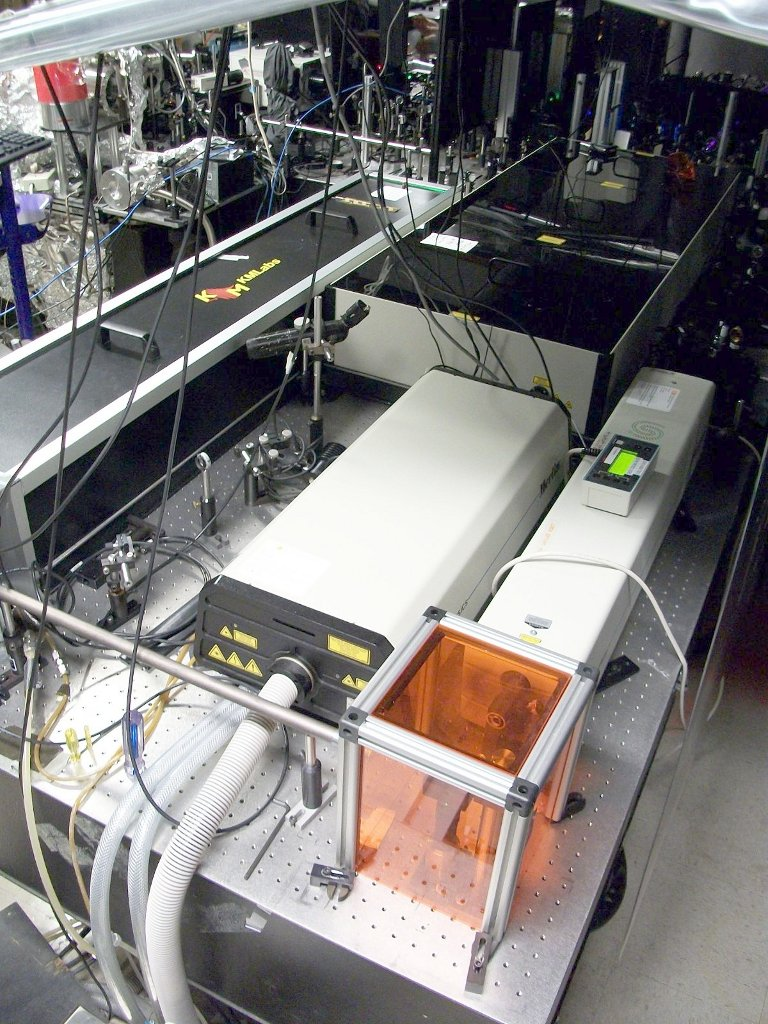
\includegraphics[height=0.8\textheight]{lasers}
\end{figure}
\end{columns}
\end{frame}

\begin{frame}
\begin{block}{Noncollinear Optical Parametric Amplifier}
\begin{itemize}
\item 760 - 515 nm (1.6 - 2.4 eV)
\item Energy: 3 - 12 $\mu$J
\item Duration: 250 fs
\item Repitition rate: 1 kHz
\end{itemize}
\end{block}
\begin{figure}
\centering
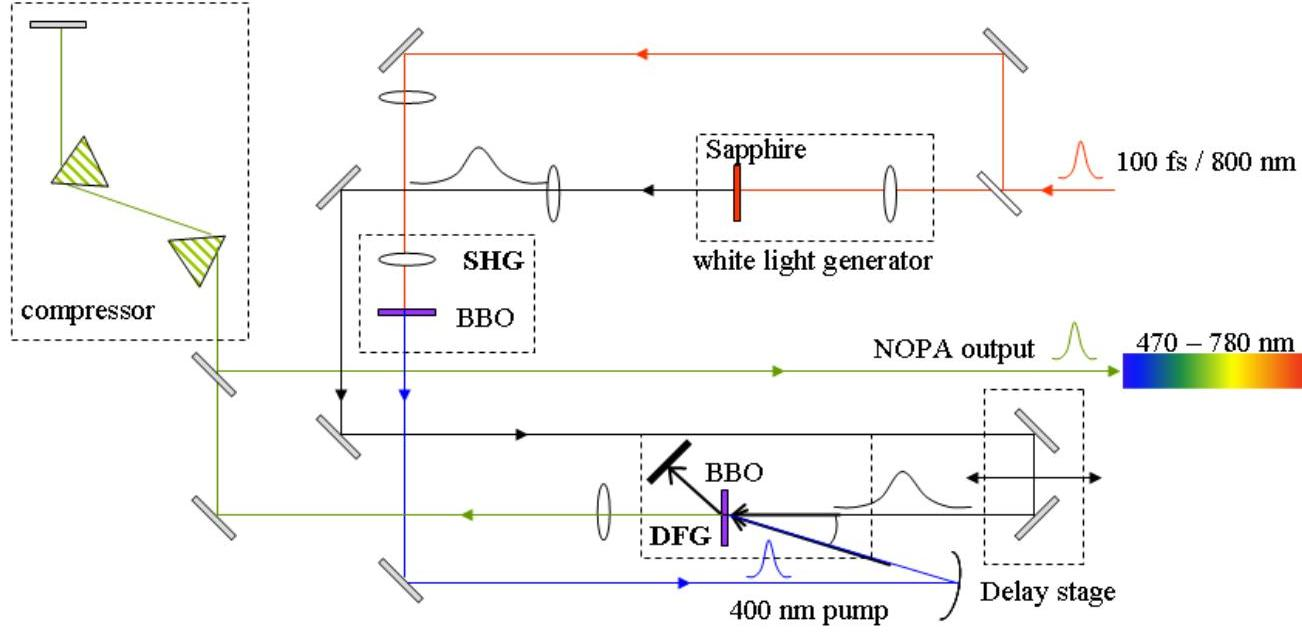
\includegraphics[height=0.5\textheight]{nopa}
\end{figure}
\end{frame}

\begin{frame}
\begin{figure}
\centering
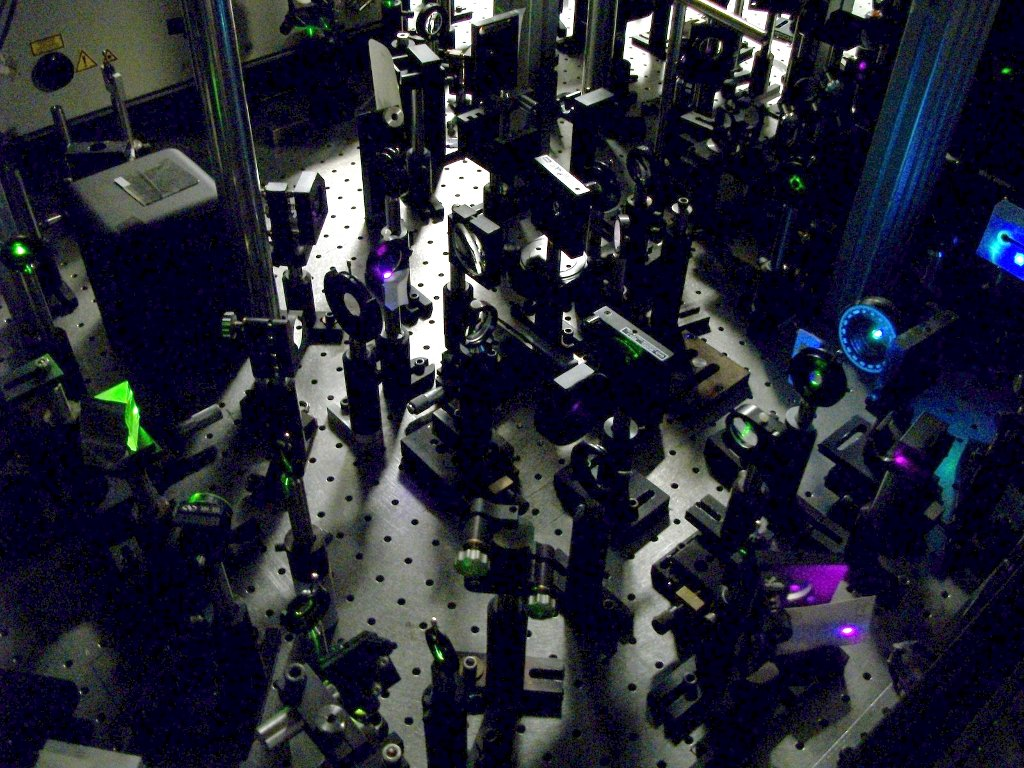
\includegraphics[width=0.8\textwidth]{nopa_pic}
\end{figure}
\begin{center}
The NOPA in action.
\end{center}
\end{frame}


\subsection{Using the XP2SHG/SFG Technique}
\begin{frame}
\frametitle{The XP2SHG/SFG Setup}
\begin{figure}
\centering
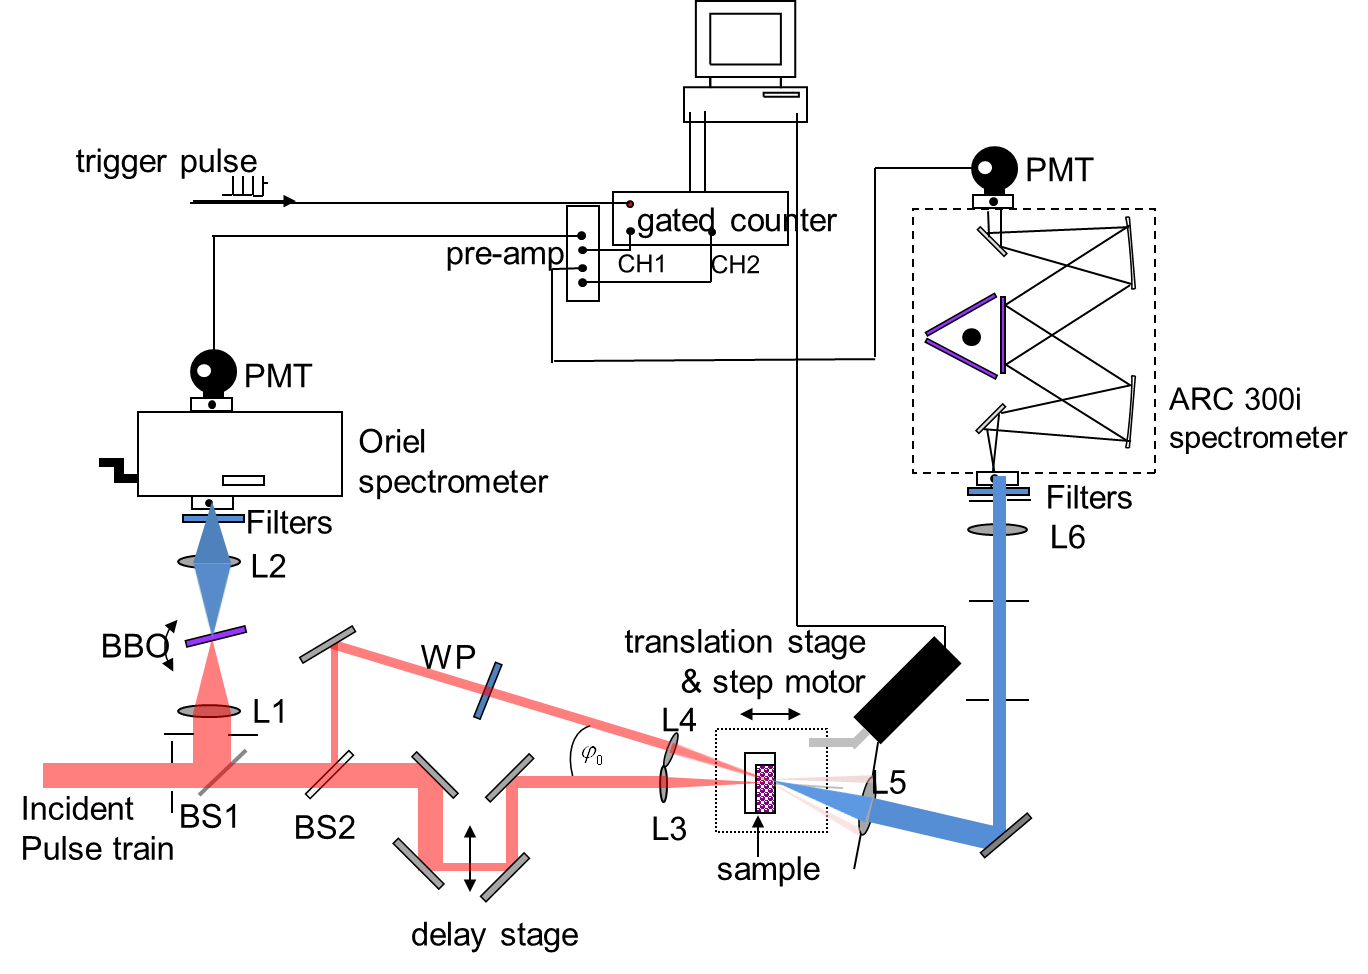
\includegraphics[width=0.8\textwidth]{xp2_diag}
\end{figure}
\begin{center}
Diagram of the XP2SHG setup.
\end{center}
\end{frame}

\begin{frame}
\begin{center}
XP2SHG using a BBO crystal.
\end{center}
\begin{columns}
\column{0.55\textwidth}
\begin{figure}
\centering
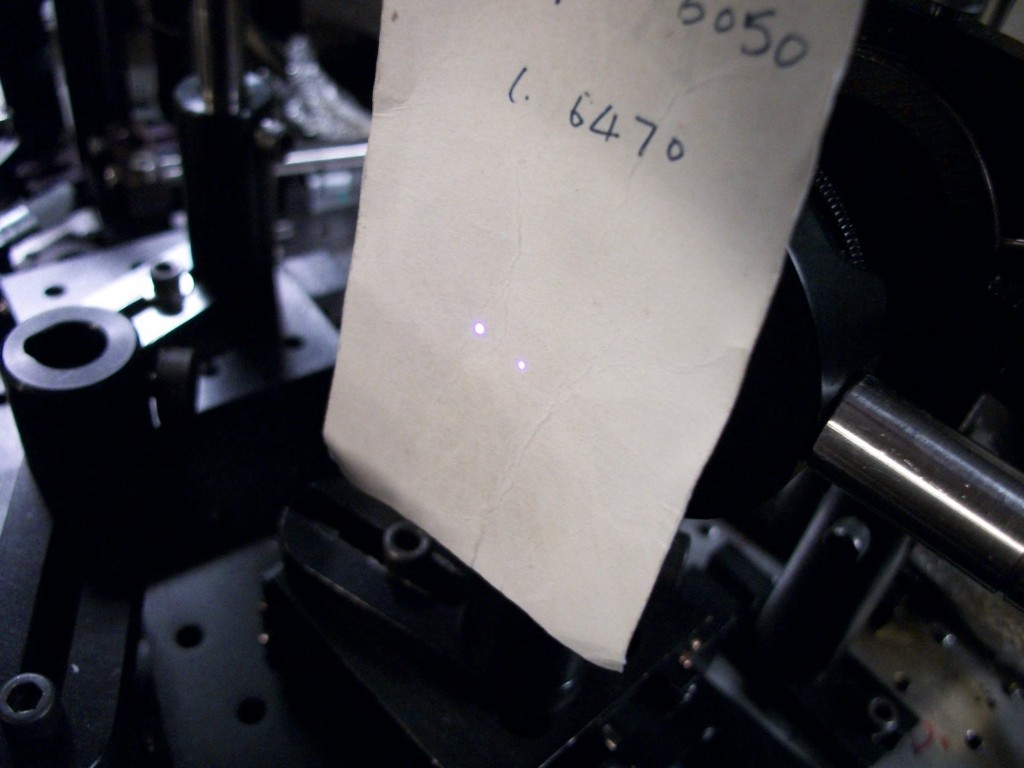
\includegraphics[width=\textwidth]{xp2_pic1}
\end{figure}
\begin{center}
Two beams in\ldots
\end{center}
\column{0.55\textwidth}
\begin{figure}
\centering
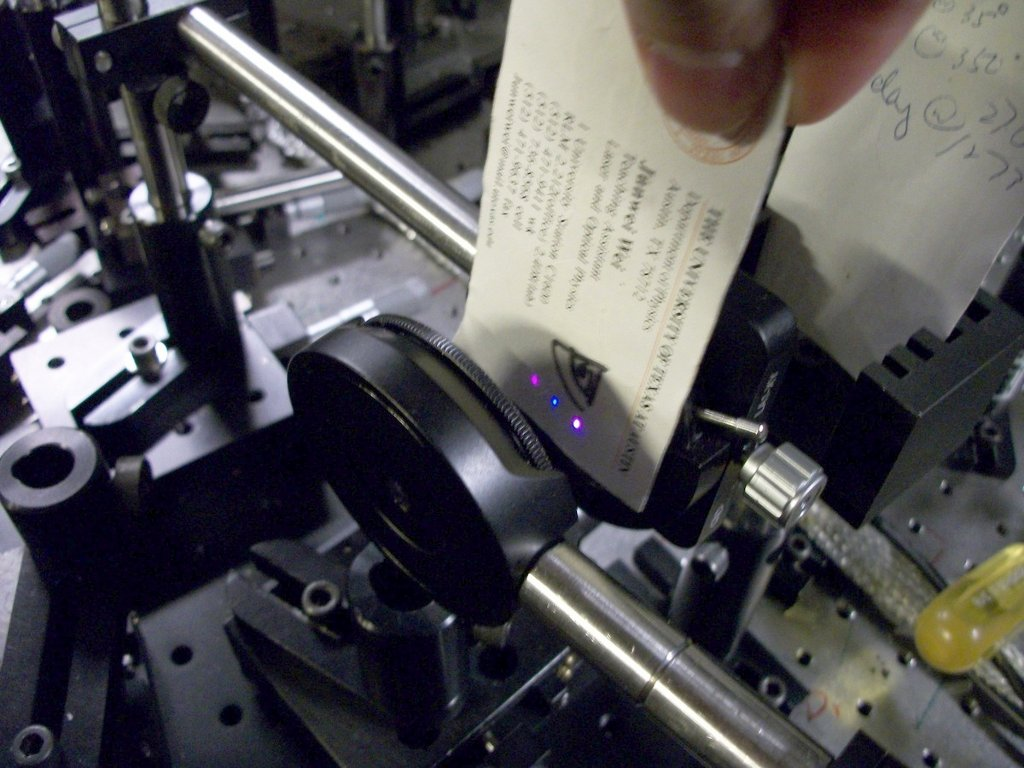
\includegraphics[width=\textwidth]{xp2_pic2}
\end{figure}
\begin{center}
three beams out!
\end{center}
\end{columns}
\end{frame}

%------------------------------ Results -------------------------------%
\section{Results}
\subsection{Linear Measurements}
\begin{frame}
\frametitle{Ellipsometry\footnote{Image: Stannered}}
\begin{figure}
\centering
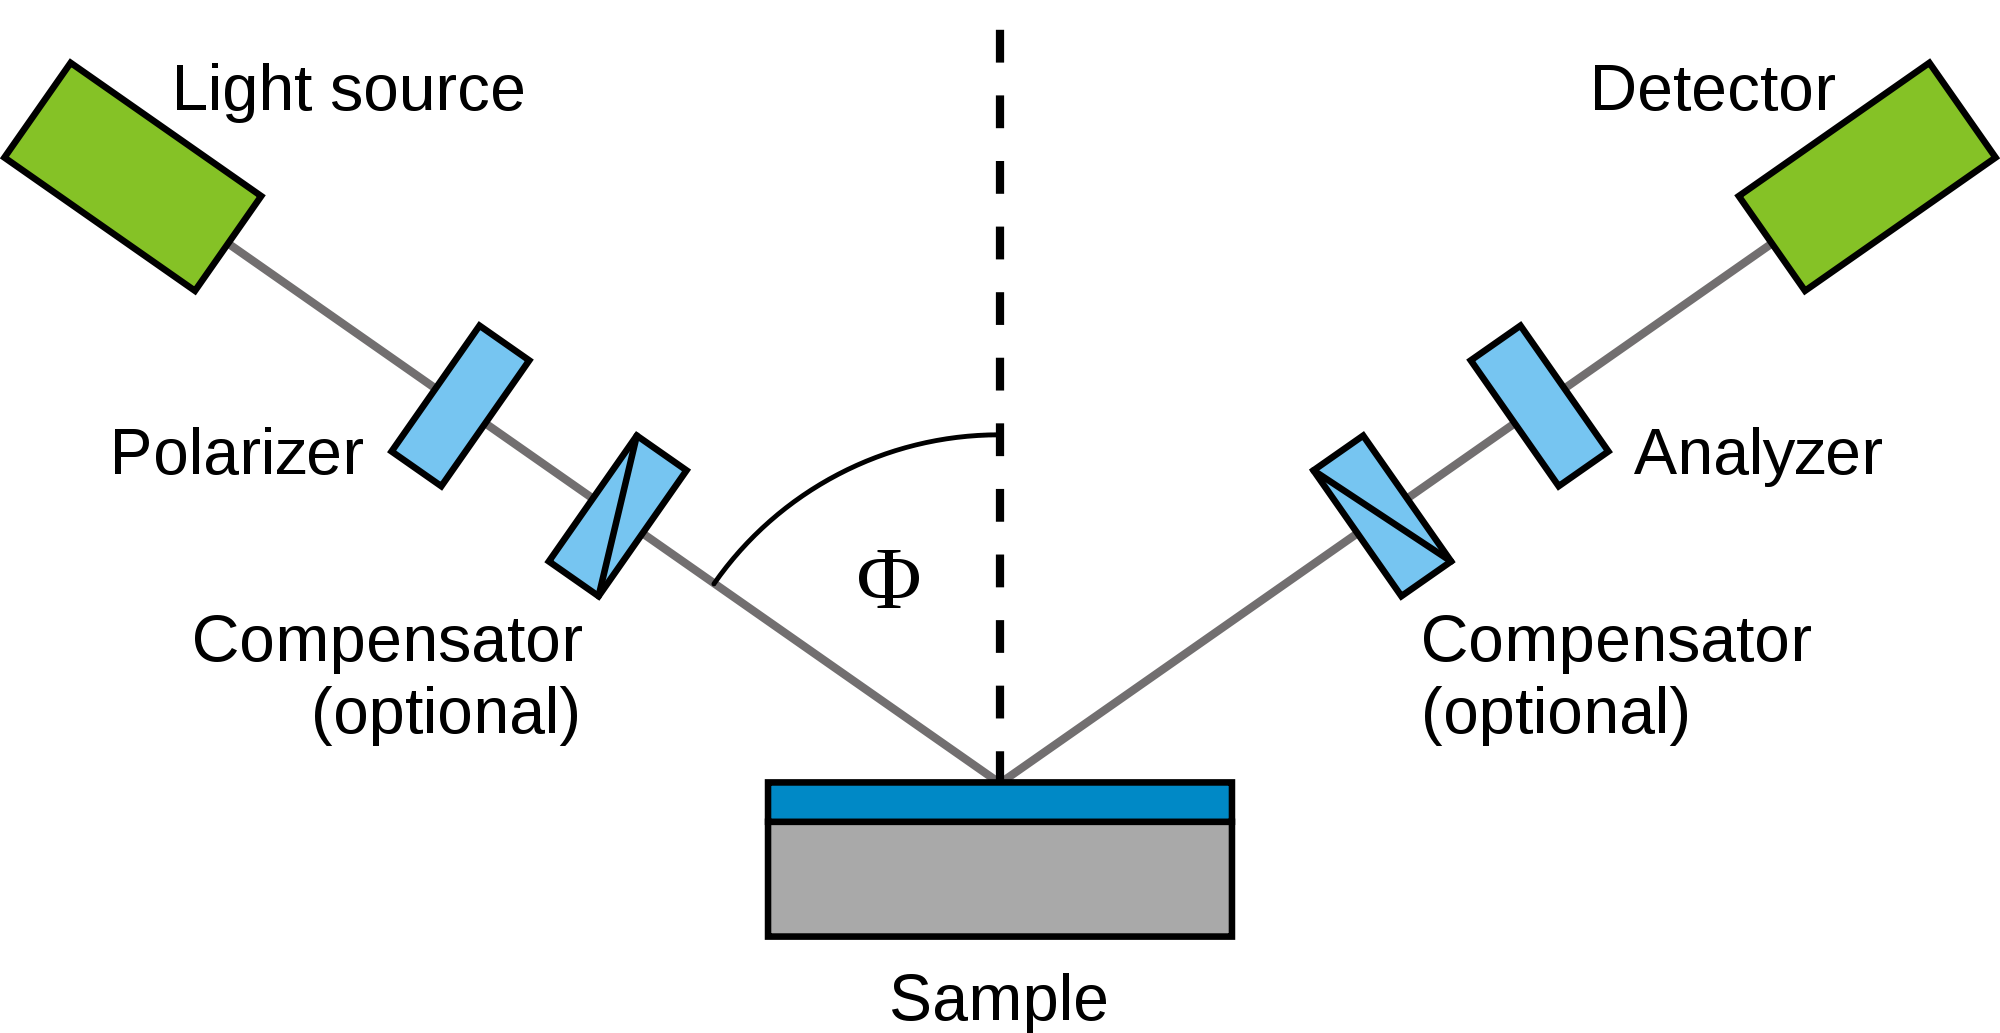
\includegraphics[width=0.77\textwidth]{ellipsometry}
\end{figure}
\begin{itemize}
\item Complement nonlinear studies and allow full characterization of nanoparticles
\item Ellipsometry can determine material dielectric function and complex index of refraction
\end{itemize}
\end{frame}

\begin{frame}
\frametitle{Linear Transmission}
\begin{figure}
\centering
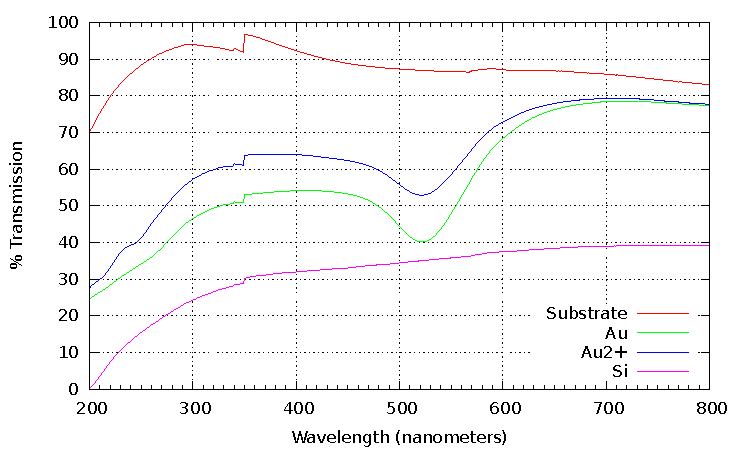
\includegraphics[width=0.77\textwidth]{linear_transmission}
\end{figure}
Gold samples have plasmon resonance around 530 nm\footnote{D.M. Schaadt et al. \emph{Applied Physics Letters}, 86:063106, 2005.} \footnote{S. Lin et al. \emph{Advanced Materials}, 17(21):2553--2559, 2005.}
\end{frame}

\begin{frame}
\frametitle{Ellipsometry -- Substrate}
\begin{columns}
\column{0.59\textwidth}
\begin{figure}
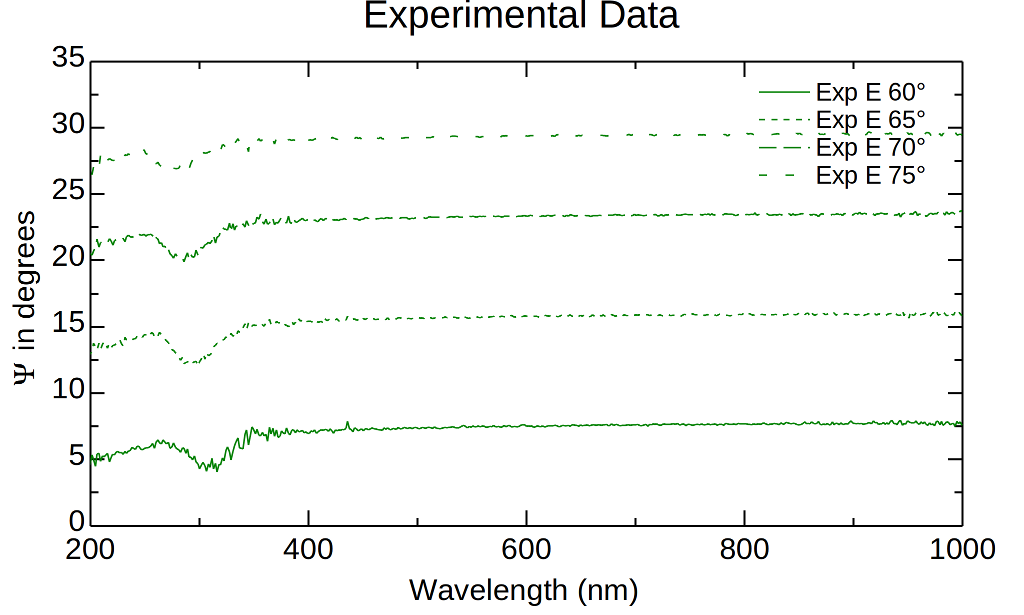
\includegraphics[width=\textwidth]{sub_ellipsometry_1}
\end{figure}
\column{0.59\textwidth}
\begin{figure}
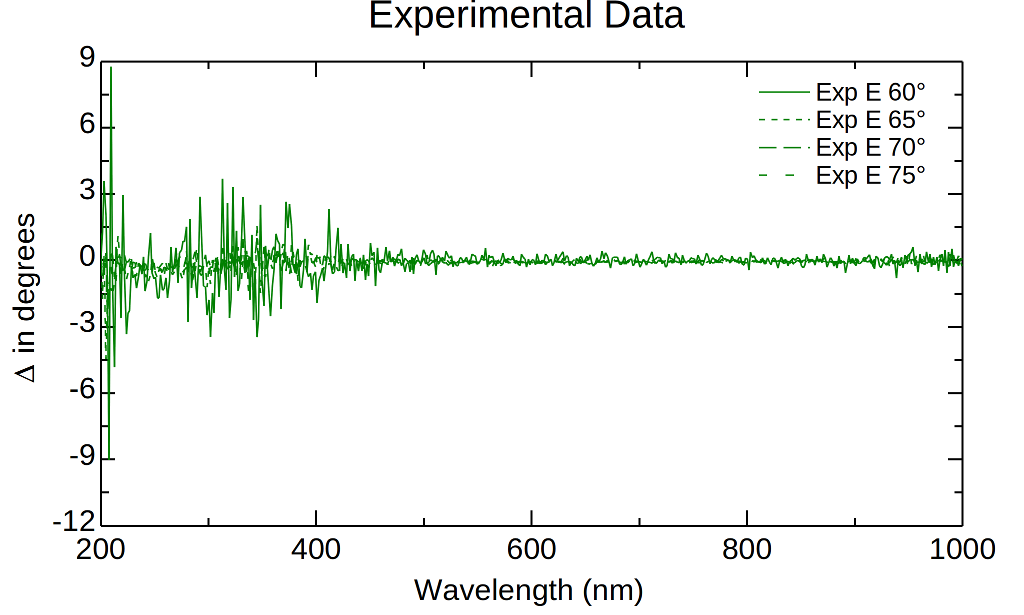
\includegraphics[width=\textwidth]{sub_ellipsometry_2}
\end{figure}
\end{columns}
\begin{center}
Graphs for $\Psi$ (left) and $\Delta$ (right).
\end{center}
\end{frame}

\begin{frame}
\frametitle{Ellipsometry -- Gold}
\begin{columns}
\column{0.59\textwidth}
\begin{figure}
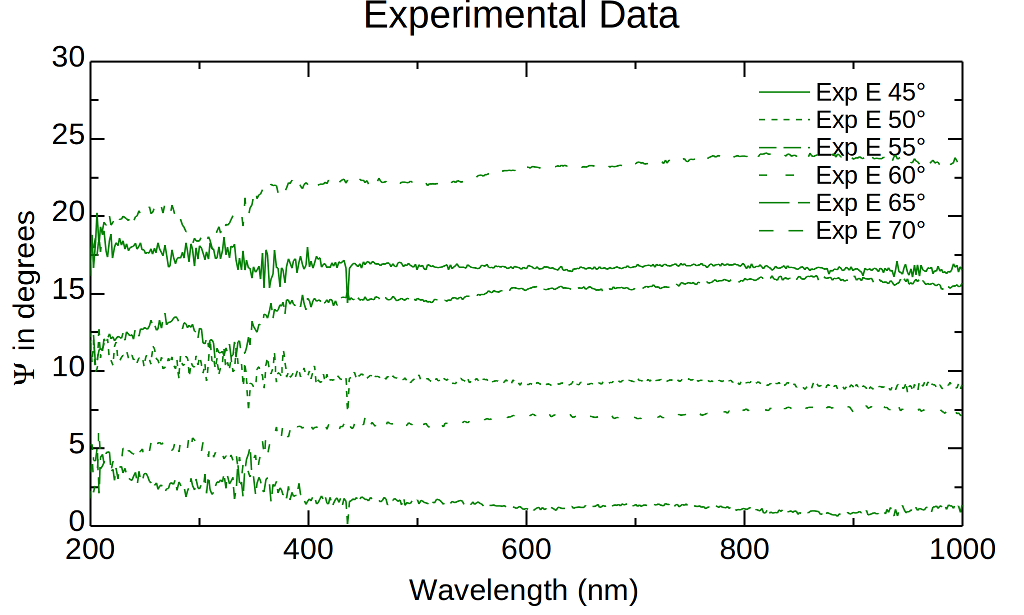
\includegraphics[width=\textwidth]{au_ellipsometry_1}
\end{figure}
\column{0.59\textwidth}
\begin{figure}
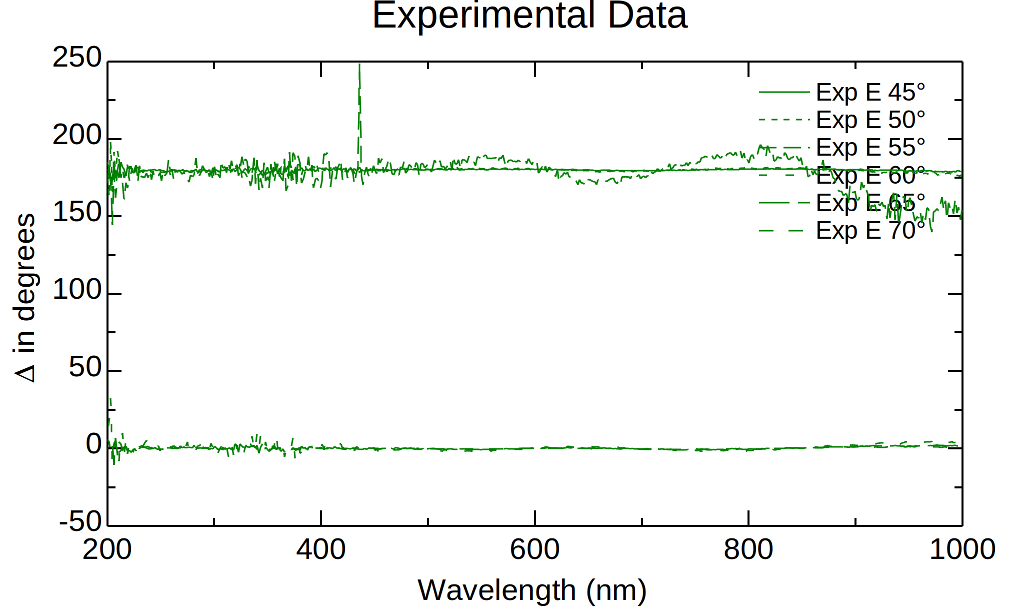
\includegraphics[width=\textwidth]{au_ellipsometry_2}
\end{figure}
\end{columns}
\begin{center}
Graphs for $\Psi$ (left) and $\Delta$ (right). Very noisy, nothing like references\footnote{H.L. Zhang et al. \emph{Advanced Materials}, 15(6):531--534, 2003.}
\end{center}
\end{frame}

\begin{frame}
\frametitle{Ellipsometry -- Silicon}
\begin{columns}
\column{0.59\textwidth}
\begin{figure}
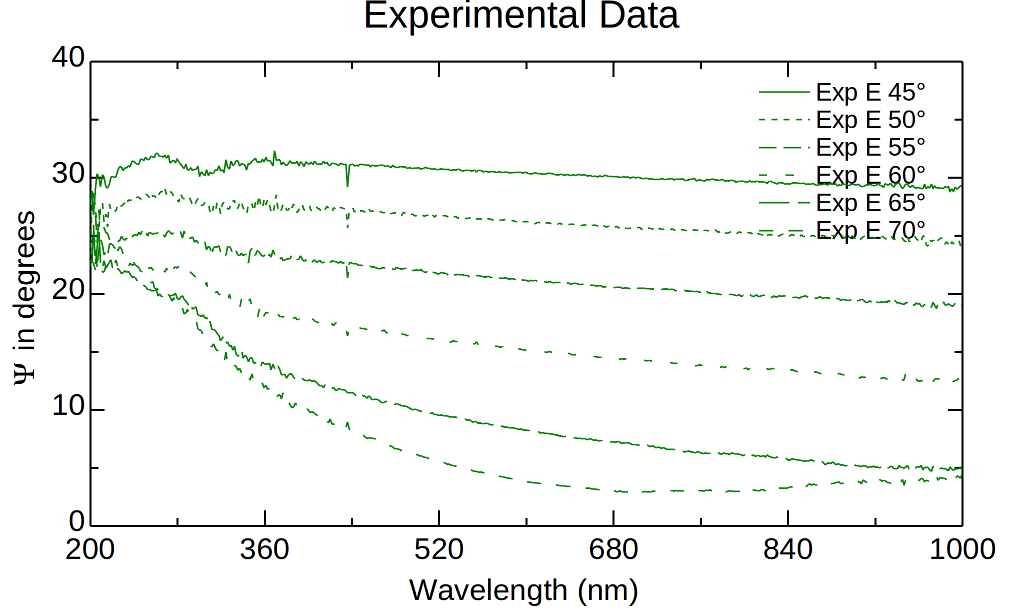
\includegraphics[width=\textwidth]{si_ellipsometry_1}
\end{figure}
\column{0.59\textwidth}
\begin{figure}
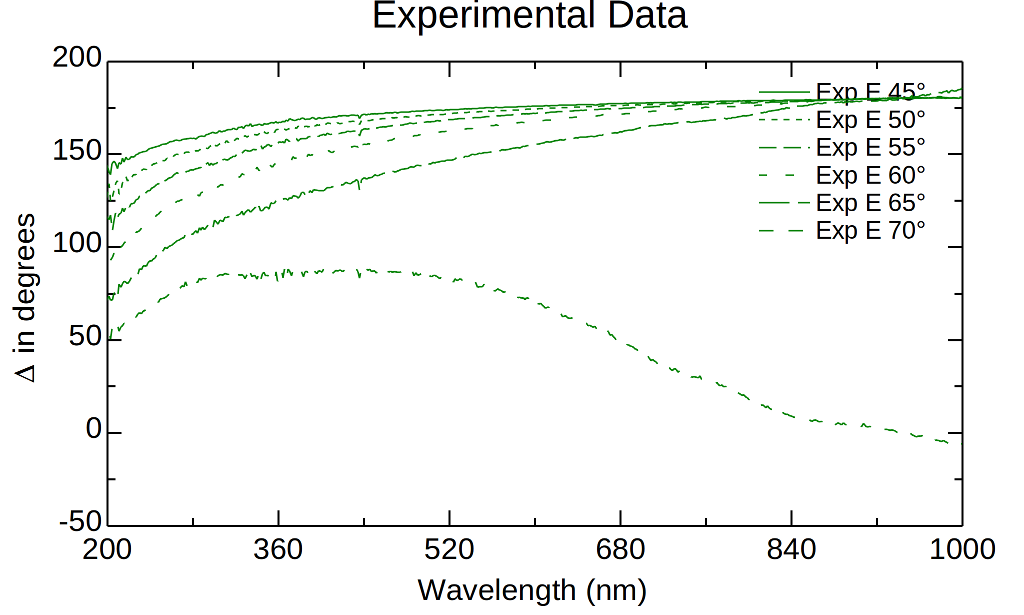
\includegraphics[width=\textwidth]{si_ellipsometry_2}
\end{figure}
\end{columns}
\begin{center}
Graphs for $\Psi$ (left) and $\Delta$ (right). Flat transmission curve for Silicon and poor ellipsometry data nothing like previous work.\footnote{J. Wei et al. \emph{Physical Review B}, 84:165316, Oct 2011.}
\end{center}
\end{frame}

\subsection{Nonlinear Measurements}
\begin{frame}
\frametitle{XP2SHG/SFG -- Substrate}
\begin{center}
Substrate XP2SFG data at 550 + 800 nm.
\begin{figure}
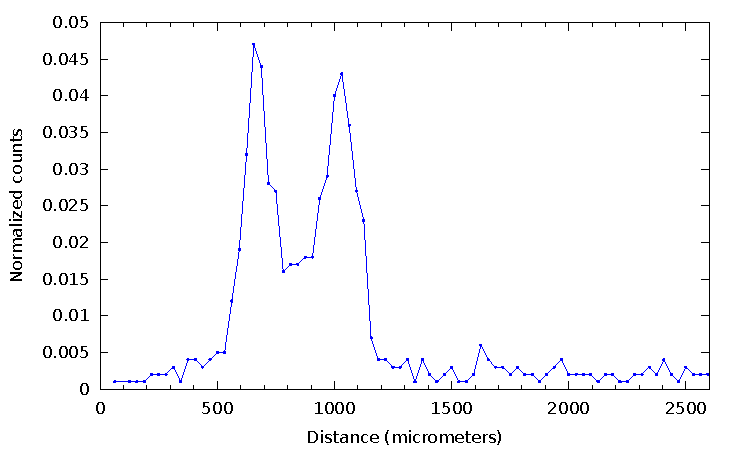
\includegraphics[height=0.5\textheight]{sub_sfg_550+800}
\end{figure}
Confirms results from previous studies\footnote{J. Wei et al. \emph{Physical Review B}, 84:165316, Oct 2011.} \footnote{A. Wirth et al. \emph{Physica Status Solidi C}, 5(8):2662--2666, 2008.}
\end{center}
\end{frame}

\begin{frame}
\frametitle{XP2SHG -- Gold}
\begin{center}
\begin{figure}
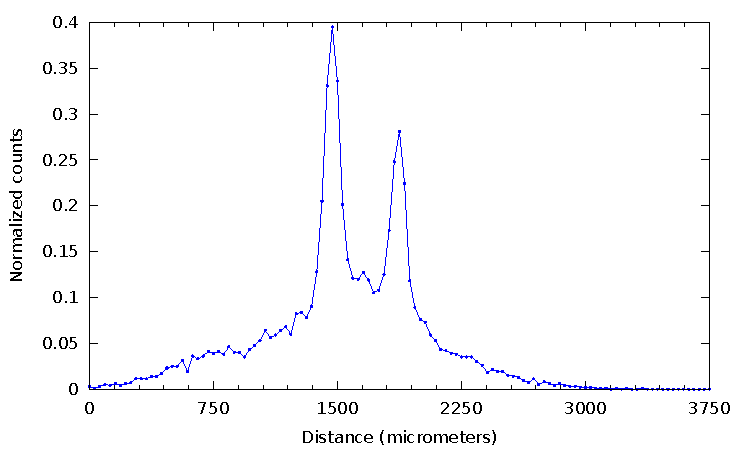
\includegraphics[width=\textwidth]{au_shg_narrow}
\end{figure}
Gold XP2SHG data, entry side.
\end{center}
\end{frame}

\begin{frame}
\begin{figure}
\centering
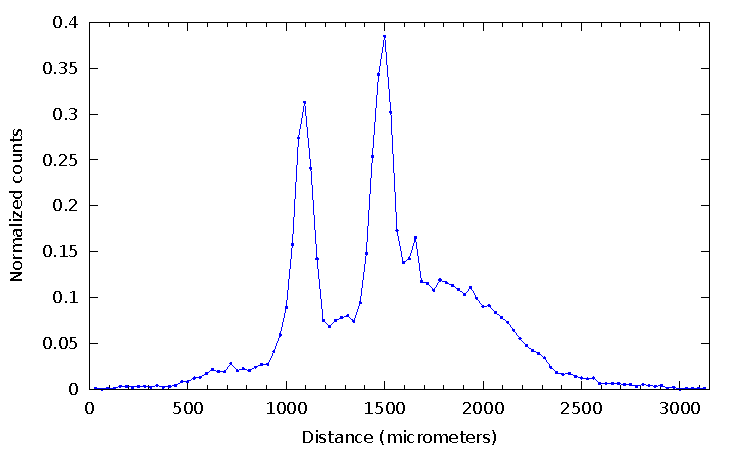
\includegraphics[width=\textwidth]{au_shg_whitelight}
\end{figure}
\begin{center}
Gold XP2SHG data, exit side.
\end{center}
\end{frame}

\begin{frame}
\begin{block}{Characteristics}
\begin{itemize}
\item Almost identical to substrate data!
\item Low input intensity produces no SHG/SFG output
\item High input intensity generates white light
\item Need to analyze entry and exit positions
\item Detector can't distinguish between single and two-beam SHG
\item Both dipolar and quadrupolar contribution
\end{itemize}
\end{block}
\end{frame}

\begin{frame}
\frametitle{XP2SFG -- Gold}
\begin{columns}
\column{0.58\textwidth}
\begin{figure}
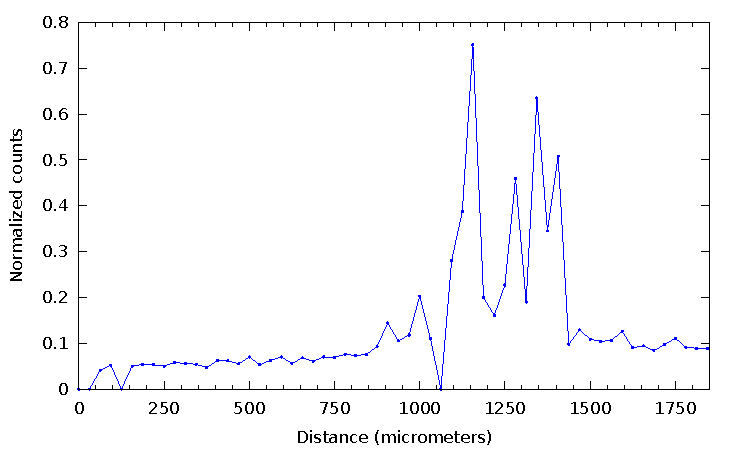
\includegraphics[width=\textwidth]{au2+_sfg_520+800}
\end{figure}
\begin{center}
Noisy signal with no discernible\\peaks at 520 + 800 nm
\end{center}
\column{0.58\textwidth}
\begin{figure}
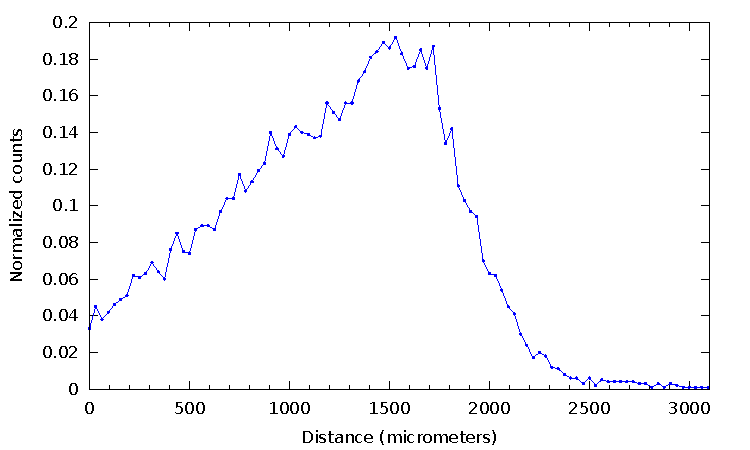
\includegraphics[width=\textwidth]{au_sfg_560+800_whitelight}
\end{figure}
\begin{center}
White light generation\\at 560 + 800 nm
\end{center}
\end{columns}
\end{frame}

\begin{frame}
\begin{center}
\begin{figure}
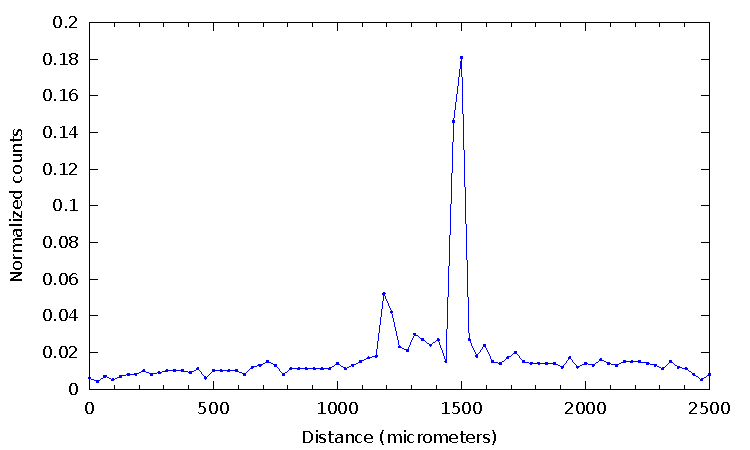
\includegraphics[height=0.55\textheight]{au_sfg_550+800_best}
\end{figure}
\end{center}
\begin{block}{Best XP2SFG data at 520 + 800 nm.}
\begin{itemize}
\item Three different frequencies: NOPA in, 800 nm in, SFG out
\item Strong output with NOPA frequency near plasmon resonance
\item Wider angle between beams should alleviate scattering
\end{itemize}
\end{block}
\end{frame}

\begin{frame}
\frametitle{XP2SHG/SFG -- Silicon}
\begin{columns}
\column{0.62\textwidth}
\begin{center}
\begin{figure}
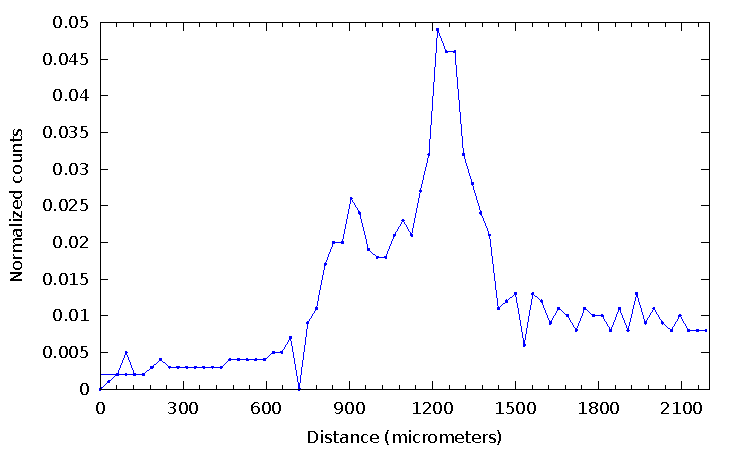
\includegraphics[width=\textwidth]{si_sfg_500+800}
\end{figure}
XP2SFG at 500 + 800 nm.
\end{center}
\column{0.55\textwidth}
\begin{itemize}
\item Weaker signal compared to Au
\item Signal not enhanced at all\footnote{J. Wei et al. \emph{Phys. Rev. B}, 84, 2011.} \footnote{A. Wirth et al. \emph{Phys. Stat. Sol. C}, 5(8), 2008.} \footnote{P. Figliozzi et al. \emph{Phys. Rev. Lett.}, 94, 2005.}
\end{itemize}
\end{columns}
\end{frame}

\begin{frame}
\frametitle{Summary}
\begin{itemize}
\item Samples of poor optical quality with massive scattering
\item Scattering and transparency to blame for erratic linear data
\item XP2SHG/SFG technique did not enhance nonlinear signal
\item Exciting near resonance may have actually been a hinderance
\item Separate Z-scans did not allow for separation of glass and nanoparticle contributions
\end{itemize}
\end{frame}


%---------------------------- Conclusions -----------------------------%
\section{Conclusions}
\begin{frame}
\begin{center}
\begin{figure}
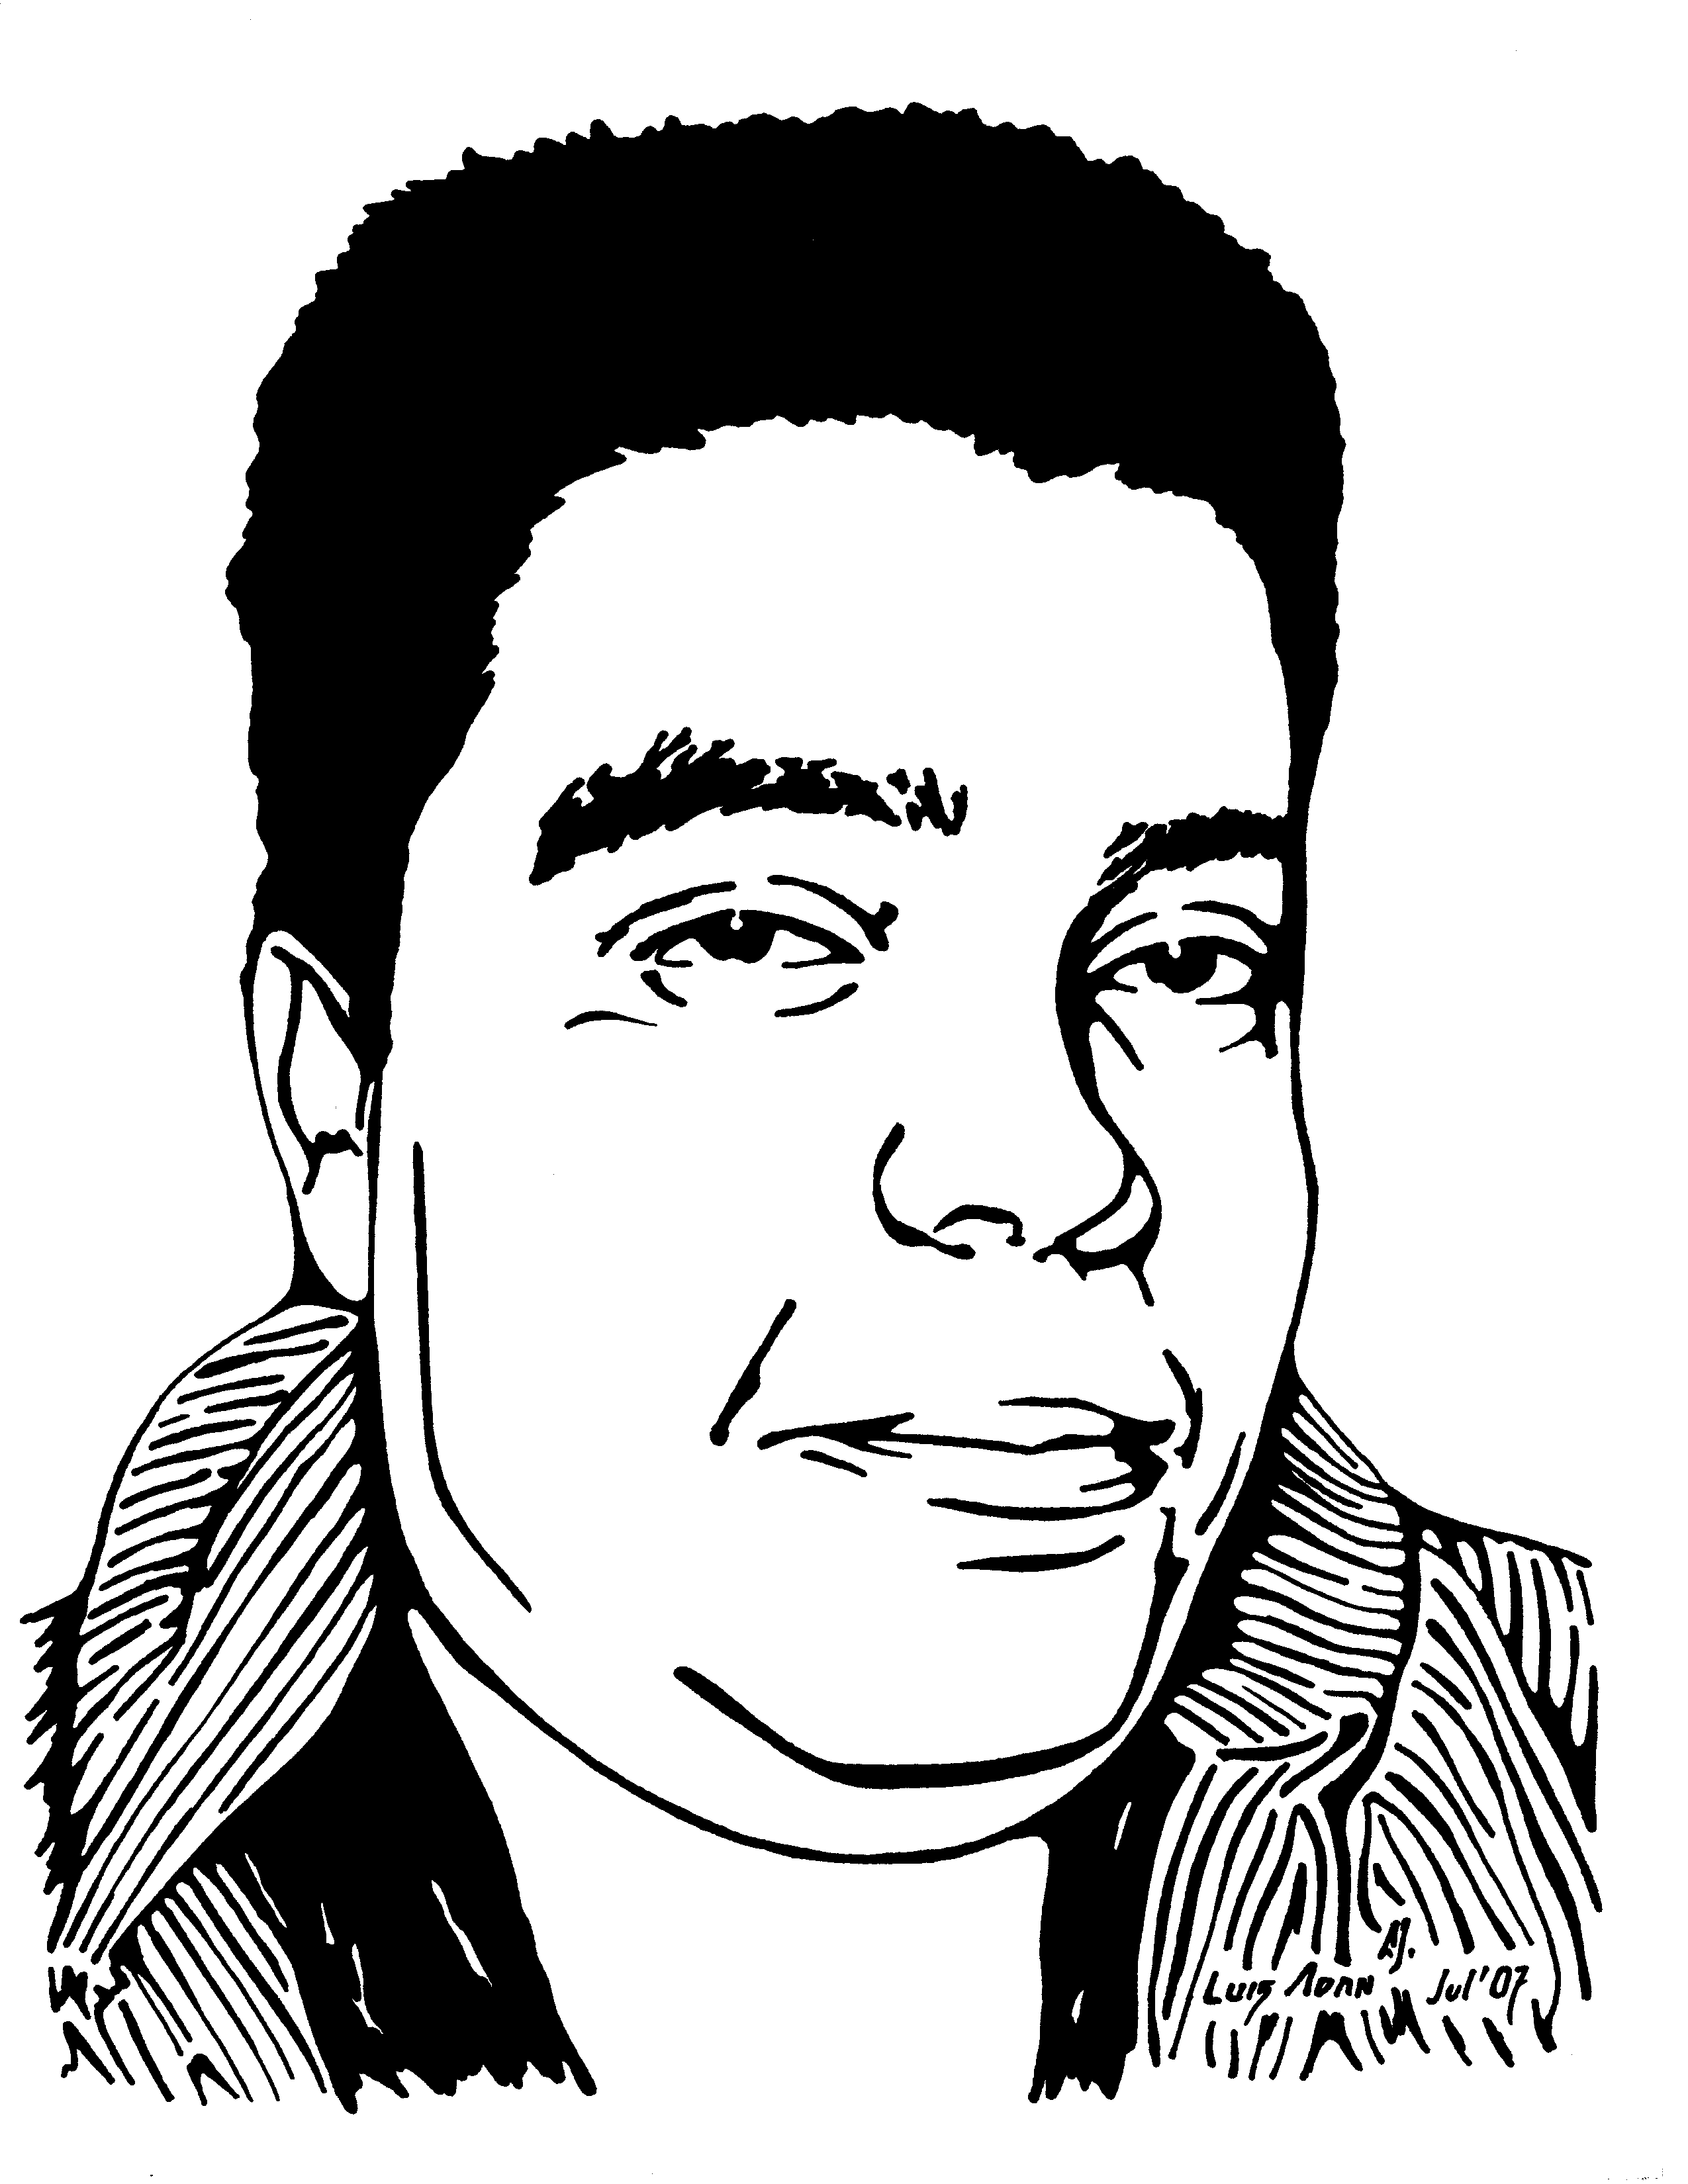
\includegraphics[height=0.87\textheight]{cabellos}
\end{figure}
{\huge ``So what?''}
\end{center}
\end{frame}

\subsection{Summary}
\begin{frame}
\frametitle{Conclusions}
\begin{block}{Accomplished}
\begin{itemize}
\item Applied the XP2SHG/SFG technique
\item Applied complementary linear measurements
\item Gained considerable experience
\end{itemize}
\end{block}
\end{frame}

\begin{frame}
\frametitle{Future Work}
\begin{enumerate}
\item Samples need to be in better shape and better characterized
\item Samples mounted on different substrates for linear measurements
\item XP2SHG/SFG technique still relatively new with metallic nanoparticles
\item Implement this setup here at the CIO
\end{enumerate}
\end{frame}

\subsection{Credits}
\begin{frame}
\frametitle{Acknowledgements}
\begin{itemize}
\item Group leaders, Dr. Ram\'on Carriles and Dr. Enrique Castro
\item Future advisor, Dr. Bernardo Mendoza
\item Dr. Mike Downer and Junwei Wei of UT Austin
\item Dr. Alejandro Reyes and Dr. Alicia Oliver of the IF-UNAM
\item DFA and all CIO staff
\item The CONACyT
\item Everyone that came to listen to this talk
\item Front page image: Travis Jennings
\item Second page images: Amanda Barnard, Vulcan 10 Petawatt
\item Dr. Cabellos drawn by Luis Ad\'an Mart\'inez
\end{itemize}
\end{frame}

\begin{frame}
\begin{center}
{\Huge !`Gracias!}\\\vspace{30pt}
!`Feliz cumplea\~nos a Alberto, Marcelo\\
\&\\
Edith\\y feliz aniversario tambi\'en!
\end{center}
\end{frame}
\end{document}
